\documentclass{controle}
\usepackage{main}

\title{Exercices : Loi binomiale}
\author{TSTMG}
\date{Chapitre 5 Partie 2}

\begin{document}

\maketitle
\thispagestyle{empty}
\bigskip

\begin{questions}

\question
On lance une pièce équilibrée 2 fois de suite.  
On note $X$ le nombre de piles obtenues.

\begin{center}
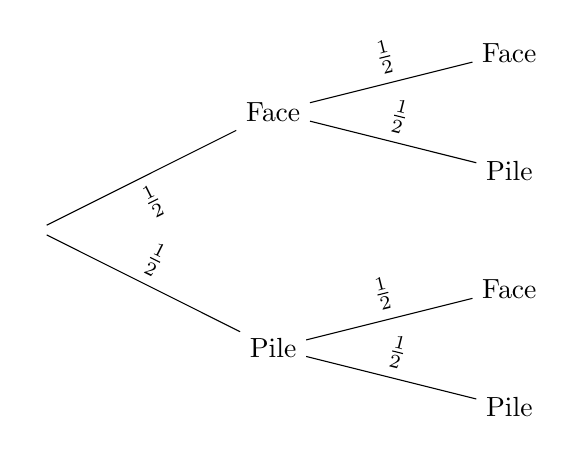
\begin{tikzpicture}[scale=1, grow=right, sloped]
\tikzstyle{level 1}=[level distance=3cm, sibling distance=3cm]
\tikzstyle{level 2}=[level distance=3cm, sibling distance=1.5cm]

\node {}
    child {
        node {Pile}
        child {
            node {Pile}
            edge from parent node[above] {$\frac{1}{2}$}
        }
        child {
            node {Face}
            edge from parent node[above] {$\frac{1}{2}$}
        }
        edge from parent node[above] {$\frac{1}{2}$}
    }
    child {
        node {Face}
        child {
            node {Pile}
            edge from parent node[above] {$\frac{1}{2}$}
        }
        child {
            node {Face}
            edge from parent node[above] {$\frac{1}{2}$}
        }
        edge from parent node[below] {$\frac{1}{2}$}
    };
\end{tikzpicture}
\end{center}

\begin{parts}
\part Calculer la probabilité que l'on obtienne une fois pile.
\part Calculer la probabilité que l'on obtienne deux fois pile.
\part En déduire la probabilité d'obtenir deux fois face.
\part Reprendre les questions précédentes en considérant le lancer de $3$ pièces. Puis $10$ pièces. Quelle est la difficulté ?
\smallskip
Pour compter le nombre de branches de l'arbre associé aux $n$ épreuves de Bernoulli comptabilisant $k$ succès, on écrit $\binom{n}{k}$.
\part À l'aide de la notation $\binom{n}{k}$, écrire la formule correspondant à la probabilité d'obtenir $Z$ piles après avoir lancé la pièce $10$ fois.
\end{parts}
\newpage

\question
Une entreprise constate que 10\% de ses clients ne paient pas leur facture à temps.
On interroge au hasard 20 clients. $X$ est la variable aléatoire comptabilisant le nombre de client mauvais payeurs

\begin{parts}
    \part Justifier que $X$ suit une loi binomiale en précisant ses paramètres.
    \part Calculer la probabilité que exactement 2 clients ne paient pas à temps.
    \part Calculer la probabilité qu'exactement 5 clients ne paient pas à temps.
\end{parts}

\bigskip

\question
Un QCM comporte 5 questions.  
Pour chaque question, une seule réponse est correcte parmi 4 proposées.
Un élève répond au hasard à toutes les questions.

\begin{parts}
    \part Quelle est la probabilité qu'une réponse soit correcte ?
    \part On note $X$ le nombre de réponses correctes. Donner la loi de $X$.
    \part Calculer la probabilité que l'élève obtienne exactement 3 bonnes réponses.
\end{parts}

\bigskip

\question
Dans une région, 15\% des foyers sont équipés de panneaux solaires.
On choisit au hasard 10 foyers.

\begin{parts}
    \part Définir la variable aléatoire $X$ et donner sa loi.
    \part Calculer la probabilité qu'exactement 2 foyers soient équipés.
    \part Calculer la probabilité qu'au plus un foyer soit équipé.
\end{parts}

\end{questions}
\end{document}
